\chapter{Anhang}


\section{Quellcodeauszug}
Im der Abbildung \ref{aircraftFamilySelectionViewModelClass} ist das vollständige ViewModel für die Auswahl des Flugzeugprogramms zu sehen. Die Klasse wurde für ein Beispiel der Navigation in der Anwendung verwendet und ist im Text referenziert.

\begin{lstlisting}[caption=Vollständige SelectAircraftFamilyViewModel Klasse für die Flugzeugprogrammauswahl]
/// <summary>
    /// This View Model has the logic for aircraft family selection. Normally its the first view if
    /// a new configuration is started.
    /// </summary>
    public class SelectAircraftFamilyViewModel : GridHolderViewModel
    {
        private AircraftModel _model;
        private ICommand _familySelectedCommand;

        public SelectAircraftFamilyViewModel()
        {
            _model = new AircraftModel();
            InitializeDataSource();
        }

        private void InitializeDataSource()
        {

            DataGroupElements = new ObservableCollection<DataCommon>
                {new AircraftProgrammGroup(_model.GetAllAircraftProgramms())}; 
        }
        public ICommand SelectAircraftCommand
        {
            get { return _familySelectedCommand ?? (_familySelectedCommand = new RelayCommand<DataCommon>(SaveSelectionAndNavigateToSummaryPage)); }
            set
            {
                _familySelectedCommand = value;
                OnPropertyChanged();
            }
        }

        private void SaveSelectionAndNavigateToSummaryPage(DataCommon data)
        {
            var selectedProgramm = GetSelectedProgramm(data.UniqueId);
            _model.SelectAircraftProgramm(selectedProgramm);
            var classToNavigate = SimpleIoc.Default.GetInstance<ISummary>();
            var navigationService = SimpleIoc.Default.GetInstance<INavigationService>();
            navigationService.Navigate(classToNavigate.GetType());
        }

        private AircraftProgramm GetSelectedProgramm(string uniqueId)
        {
            return _model.GetAllAircraftProgramms().FirstOrDefault(programm => programm.UniqueId.Equals(uniqueId));
        }
    }
\end{lstlisting} 
\label{aircraftFamilySelectionViewModelClass}

 
\section{Evaluationsbögen} \label{anhangEva}
Die Fragebögen für die Experten und die Benutzer sind auf den folgenden beiden Seiten angehängt.

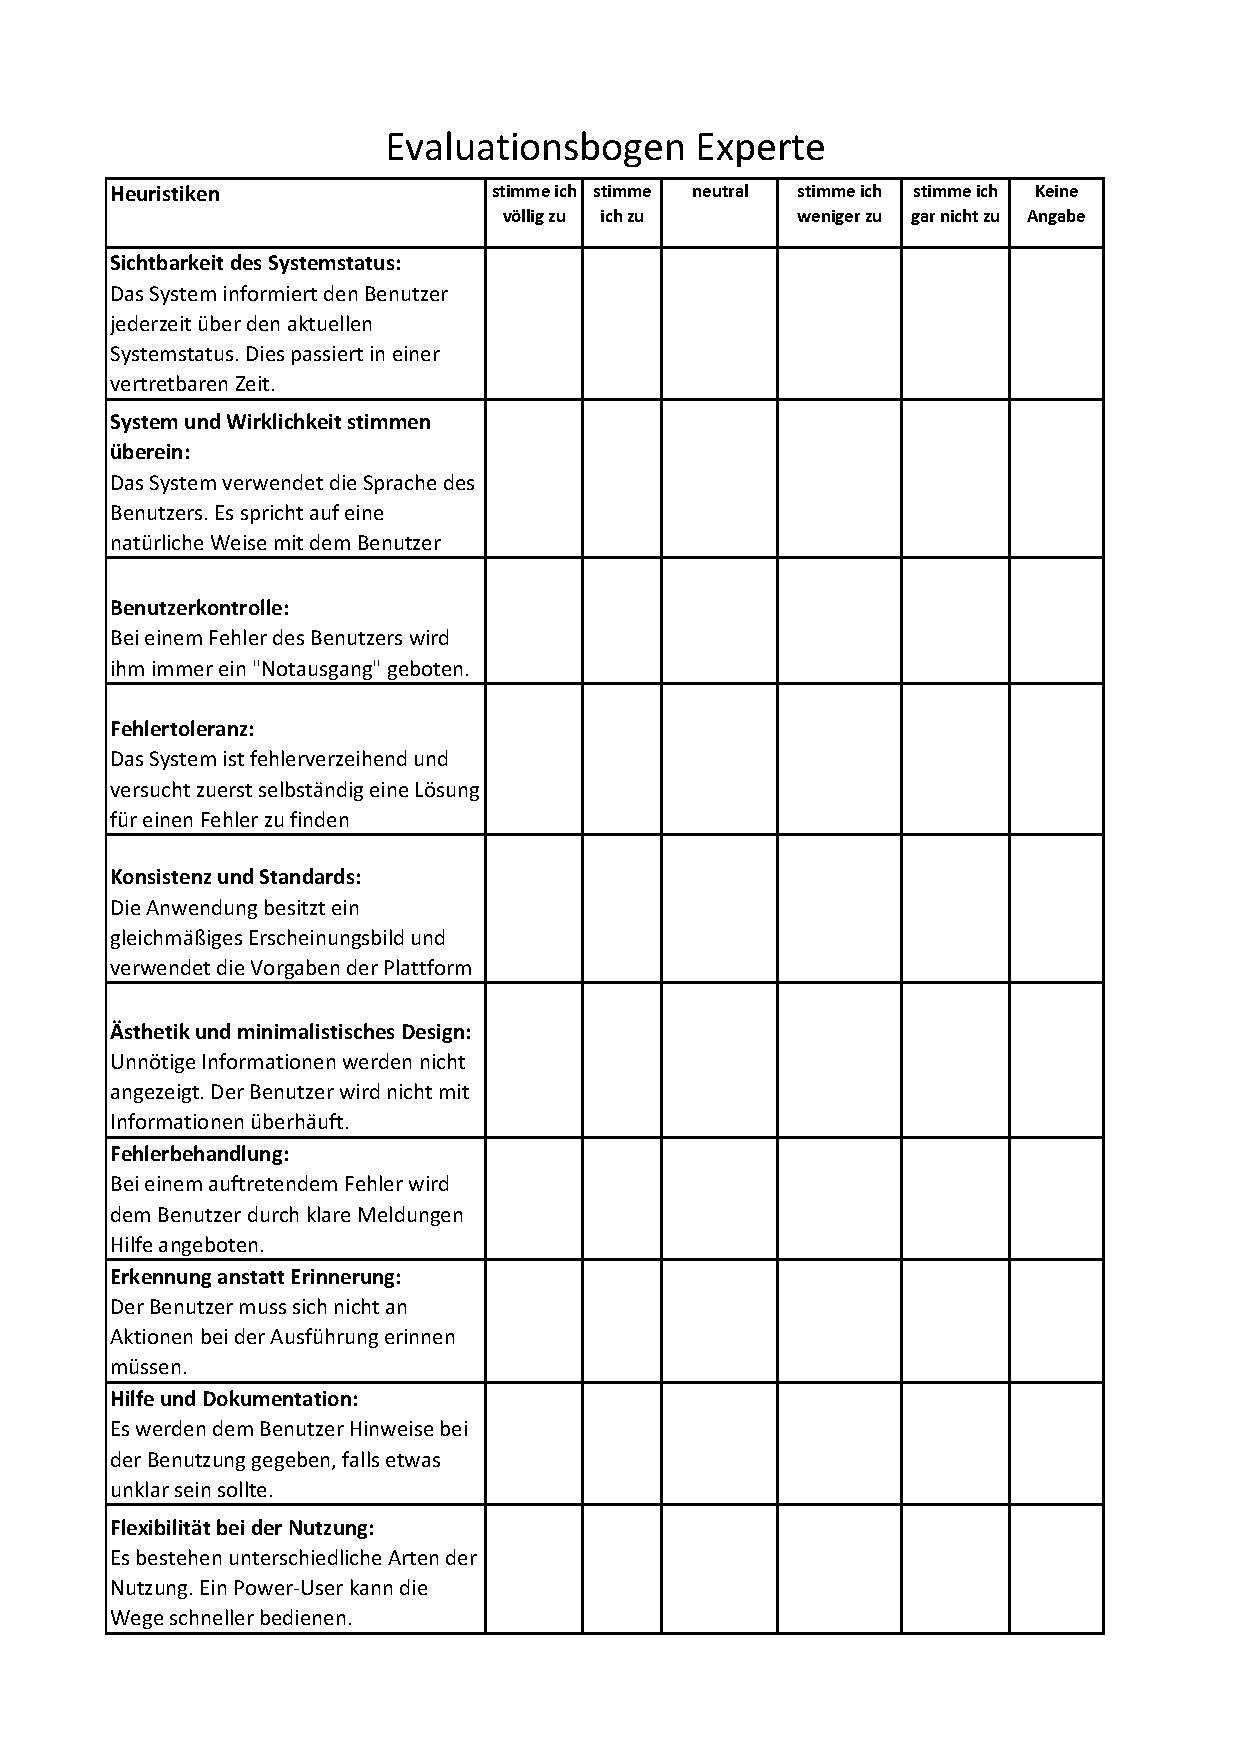
\includepdf[pages=1]{anhang/evaluationsbogenExperte.pdf}
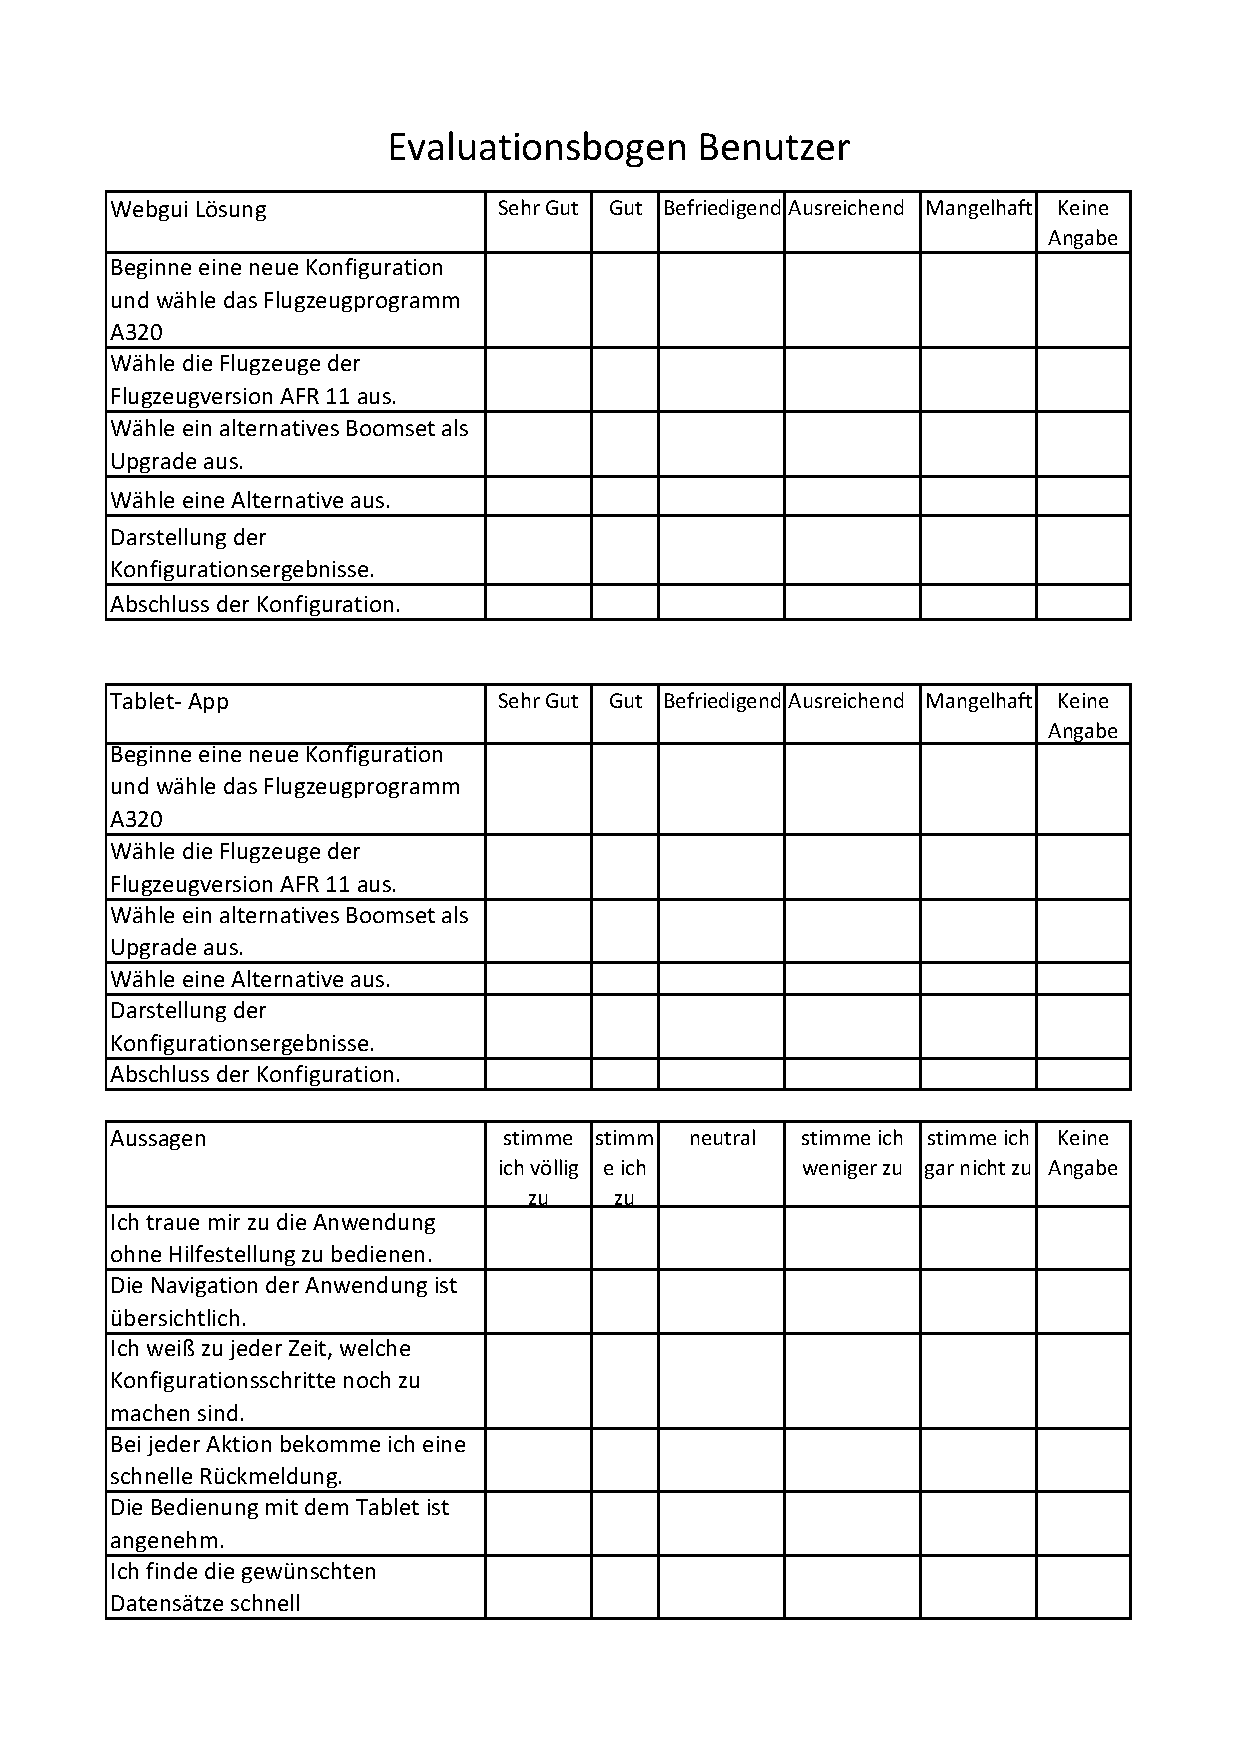
\includepdf[pages=1-2]{anhang/evaluationsbogenUser.pdf}

\section{Evaluationsergebnisse} \label{anhangEvaErg}
Im Folgenden werden die kompletten Ergebnisse der Evaluation dargestellt. In Abbildung \ref{bewertungWebguiComplete} ist die vollständige Auswertung der Fragebögen für die Fragen zur vorhandenen Konfigurationslösung. Das Ergebnis wurde zur Unterscheidung der beiden Lösungen verwendet. Die vollständigen Ergebnisse der Fragen mit dem Schwerpunkt für die Erfüllung der Nicht-Funktionalen Anforderungen ist im Diagramm \ref{tabletComplete} zu sehen. Das vollständige Ergebnis der Expertenbefragung zu den Heuristiken nach Nielsen ist in der Abbildung \ref{bewertungExpertComplete} dargestellt. \par 
\begin{figure}[H]
\centering
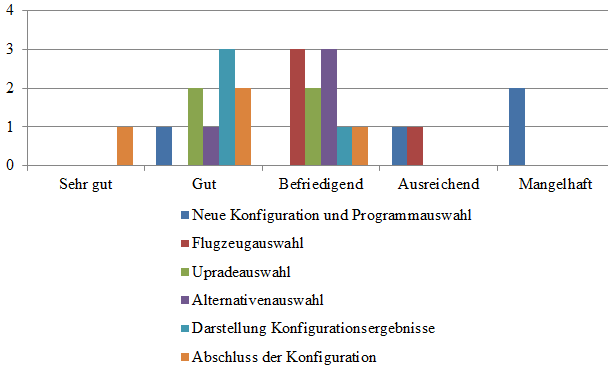
\includegraphics[width=\hsize]{images/bewertung_webgui}
\caption{Ergebnis der Fragen zur vorhandenen Konfigurationslösung}
\label{bewertungWebguiComplete}
\end{figure}
\begin{figure}
\centering
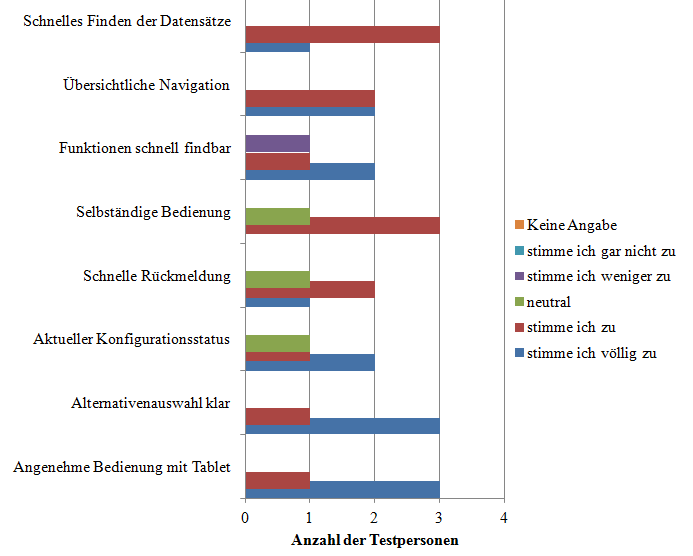
\includegraphics[width=\hsize]{images/bewertung_tabletComplete}
\caption{Vollständiges Ergebnis der Benutzerumfrage zu Usability Fragen}
\label{bewertungTabletComplete}
\end{figure}
\begin{figure}
\centering
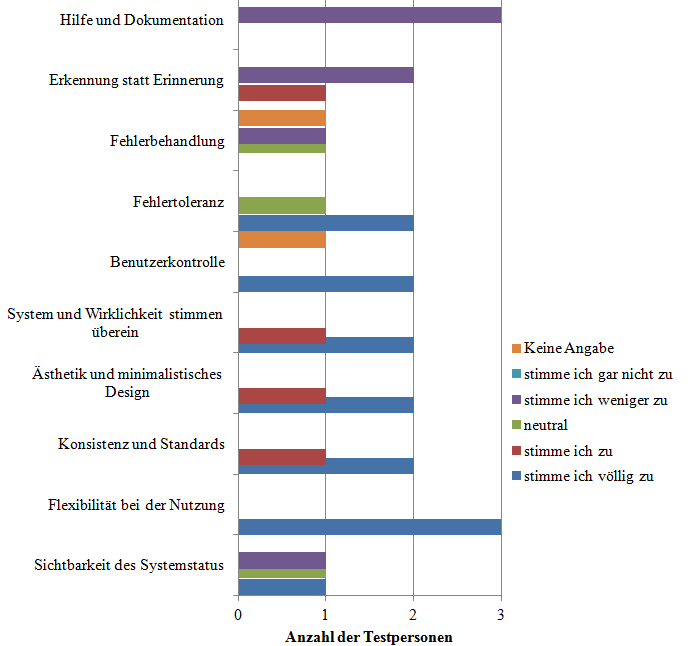
\includegraphics[width=\hsize]{images/bewertung_expert_complete}
\caption{Vollständiges Ergebnis der Expertenbefragung}
\label{bewertungExpertComplete}
\end{figure}